
\section{Die Idee der linearen Regression}
\label{RegressionsIdee}
Ziel der Regression ist es, den funktionalen Zusammenhang $Y =
f(X_{1} ,X_{2} ,...,X_{N} )$ zwischen den
Eingangs-Messgrößen $X_{i}$ (Regressor) und der Ausgangsgröße $Y$
(Regressanden) möglichst gut zu charakterisieren.

Der allgemeinste Fall der Regressionsrechnung ist der mit sowohl mehreren
Regressoren als auch mehreren Regressanden.
Regressionsrechnung mit einem Regressanden, wird \textbf{univariate Regression}, oder oft einfach nur lineare Regression genannt.
Die Darstellung der Modellgleichung kann dabei wie folgt aussehen 
\begin{equation}
Y_j = f(X_{1,j},\dots, X_{i,j},\dots, X_{N,j}) + \varepsilon_j \quad \mathrm{mit} \quad j = 1,2,\ldots,J
\label{Kap2Modellglunivar}
\end{equation}
wobei $Y_j$ eine Beobachtung zur Zufallsgröße, dem Regressanden $Y$, darstellt bei Vorgabe (Einstellung an einem
Gerät wie im Beispiel von Kapitel 1 der Präzisionsstromquelle) $X_{i,j}$ des Regressors $X_i$.
Wenn es mehrere abhängige Größen, also mehrere Regressanden gibt, spricht man von \textbf{multivariater Regression}. Die Regressoren müssen voneinander \textbf{linear unabhängig} sein.
Sie können aber auch eine Potenzbeziehung zueinander haben, also quadratisch, kubisch etc.
Wir werden für die Methode der Regressionsrechnung zur Schätzung von Polynomkoeffizienten
eine Eingangsgröße $X$ und eine Ausgangsgröße $Y$ betrachten, die über ein Potenzgesetz
\begin{equation}
Y = f(X) \propto X^k \quad \mathrm{mit} \quad k \in I \! \! N_0
\label{potenzgesetzlinReg}
\end{equation}
also mit $k$ als natürliche Zahl einschließlich der Null, verknüpft sind.

Bei der Regressionsrechnung wird vorausgesetzt,
dass der Regressor $X$ eine Größe ist, die voreingestellt ist und keiner Streuung unterliegt,
und nur der Regressand $Y$ streut und deshalb als Zufallsgröße betrachtet wird.
Die Streuung kann verschiedene Ursachen haben:
\begin{itemize}
\item Die indirekten Messgrößen, hier die Größen, die durch die
Modellparameter beschrieben werden, streuen aufgrund von nicht im Modell
enthaltenden Einflüssen.
Das bedeutet, dass das Modell eine Approximation des physikalischen Sachverhalts ist.
\item Der Messvorgang des Regressanden führt zu Streuungen.
\end{itemize}
Die Modellparameter sind also wie die Regressanden als Zufallsvariablen
zu betrachten. Die Regression soll nun Schätzwerte für die
Modellparameter liefern. Das Modell wird über einen 
funktionalen Zusammenhang zwischen Regressor und Regressand 
\begin{equation}
Y = f(X)
\label{Kap2Modellgleichung}
\end{equation}
beschrieben.

Um eine Schätzung für die Parameter des funktionalen Zusammenhangs $Y = f(X)$
zu erhalten, wird die Eingangsgröße in einem bestimmten Bereich
variiert. Man misst $J$ Messwertpaare $(X_j ,Y_j )$ mit $j=1,\ldots, J$, die sich als Punktwolke in einem Diagramm darstellen lassen. Auf Grund der Streuungen werden die Wertepaare $(X_j, Y_j )$
die Gleichung $Y_j = f(X_j )$ nicht exakt erfüllen,
sondern etwas abweichen $\varepsilon_j$, d.~h.
\begin{equation}
Y_j = f(X_j) + \varepsilon_j \quad \mathrm{mit} \quad j = 1,2,\ldots,J
\label{Kap2ModellglmitResiduen}
\end{equation}

Wir stellen hier zusammen welche Typen von Größen bei der Regressionsrechnung behandelt werden:
\begin{itemize}
	\item Die unabhängigen Größen $X$ werden
	 vorgegeben. Sie haben genau bekannte Werte (engl.\ \textsl{exactly known values})
	und sind somit keine Zufallsgrößen. Sie sind unabhängig und 
	heißen \textbf{Regressoren}.
	\item Die abhängigen Größen $Y$, d.h.\ die \textbf{Regressanden} streuen und ihre Residuen sind
	normalverteilt mit Erwartungswert $E(\varepsilon) = 0$ und Varianz $\mathrm{Var}(\varepsilon) = \sigma^2$. 
	
	Die Residuen sind \textbf{unabhängig und identisch verteilt}, kurz u.i.v.
	\begin{equation}
	\varepsilon \; \overset{u.i.v.}{\sim} \; \mathcal{N}(0,\sigma_{\varepsilon}) .
	\label{Resinormalverteilt}
	\end{equation}
	Die Regressanden werden auf Grund ihrer Streuung als Zufallsgrößen betrachtet.
	Zu jedem beobachteten Wert des Regressanden wird jeweils ein Regressorwert
	zugeordnet (engl. \textsl{observed data corresponding to the known values}).
	Sie sind abhängig vom Regressor und werden deshalb auch \textsl{dependent variable} oder
	\textsl{response variable} genannt.
	\item Modellparameter, die unbekannt sind (\textsl{unknown parameters}), sind Zufallsgößen. Sie werden
	auch Regressionsparameter (\textsl{regression parameters}) genannt.
	\item Ferner gibt es zusätzliche unbekannte Parameter, und zwar die Varianzen der beteiligten
	Zufallsgrößen, \textsl{unknown additional parameters}. % $\boldsymbol{\delta}$ (unknown variance parameters)
\end{itemize}
	
\begin{figure}
	\begin{center}
		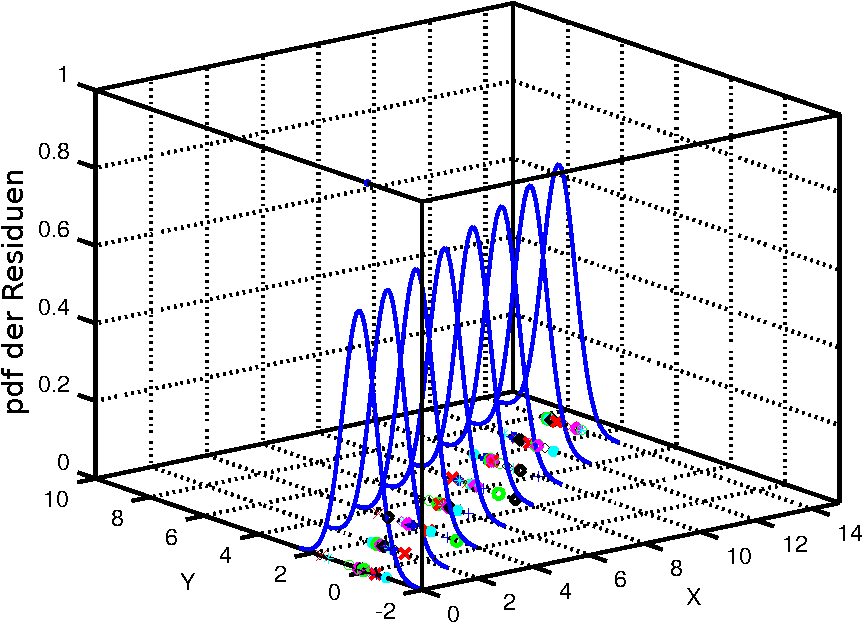
\includegraphics[width=100mm]{02_vorlesung/media/regressionNormalResi_1b.pdf}
		\caption{\label{regressionNormalResi} Lineare Regression für unabhängig und
			identisch verteilte Residuen.}
	\end{center}
\end{figure}

Abb.~\ref{regressionNormalResi} veranschaulicht, dass die Residuen normalverteilt sind, wobei die vertikale Achse die Wahrscheinlichkeitsdichte der Residuen darstellt. Der englische Begriff für Wahr\-schein\-lich\-keits\-dichte\-ver\-teil\-ung ist \textsl{probability density function}, kurz pdf. Die unterschiedlichen
Farben und Symbole sollen unterschiedliche Durchläufe gleicher Messvorgänge darstellen.

\section{Lineare Regression als Beispiel zur Methode der kleinsten Abweichungsquadrate}
Man bestimmt die Parameter der Regressionsfunktion $Y =
f(X)$ nun so, dass die Summe der Quadrate der
Abweichungen der Datenpunkte vom Modell (\textbf{Residuen}) $\varepsilon_j $ möglichst klein wird
(Methode der kleinsten Abweichungsquadrate),
d.h.\ die \textbf{Kostenfunktion} $Q$ muss minimal werden:
\begin{equation}
Q: = \sum\limits_{j = 1}^J {\varepsilon_j ^2 = } \sum\limits_{j = 1}^J {(Y_j
	- f(X_j ))^2 \to } \,\,\min
\label{eq:Minimimierung-kleinster-Fehlerquadrate}
\end{equation}
Die Kostenfunktion ist ein Maß für die Abweichung der Messgrößen vom Modell in Abhängigkeit von der
Wahl der Werte für die Modellparameter. Für gegebene Werte für die Modellparameter liefert die
Kostenfunktion ein Maß für die Qualtität der Schätzung und wird \textbf{Qualitätsmaß} genannt.

Wie in Kapitel 1 dargelegt, basiert dies auf dem Maximieren der Likelihood, der
normalverteilten bzw.\ gaußverteilten Wahrscheinlichkeitsdichte der Residuen. Da diesem Verfahren
die Annahme als Voraussetzung zugrunde liegt, dass die Likelihood gaußverteilt ist, spricht man in der
ingenieurmäßigen Anwendung auch vom Ausgleichsverfahren nach Gauß.

In die Modellgleichung (\ref{Kap2Modellgleichung}) setzen wir mehrere Potenzgesetze (\ref{potenzgesetzlinReg})
ein, um folgenden Polynomansatz aufzustellen
\begin{equation}
Y = f(X) \equiv p_m = \theta _m X ^m + \theta _{m-1} X^{m - 1} + 
\cdots + \theta _1 X + \theta _0
\end{equation}
$m$ bezeichnet den Grad des Polynoms. Die Anzahl der Regressionsparameter bezeichnen wir mit $M = m+1$.
Unter Berücksichtigung der Streuung der Beobachtungen $Y_j$ des Regressanden ist dies wie in Gl.~(\ref{Kap2ModellglmitResiduen})
\begin{equation}
Y_j = f(X_j) \equiv p_m = \theta _m X_j^m + \theta _{m-1} X^{m - 1} + \cdots + 
\theta _1 X_j + \theta _0 + \varepsilon_j
\end{equation}

Für die Schätzung der Polynomkoeffizienten setzen wir den Polynomansatz in die 
Minimumbedingung Gl.~(\ref{eq:Minimimierung-kleinster-Fehlerquadrate}) ein:
\begin{equation}
Q = Q(\theta _m ,\theta _{m - 1} ,\ldots ,\theta _1 ,\theta _0 ) =
\sum\limits_{j = 1}^J {(Y_j - p_m (X_j ))^2 \to } \,\,\min
\end{equation}

Die Schätzwerte der Koeffizienten $\hat{\theta}_k$, für die die Kostenfunktion $Q$ ein Minimum annimmt, sind
die beste Schätzung oder das Optimum der Parameter $\theta _k $, weshalb im englischen Sprachgebrauch auch der Begriff
\textsl{best fit} Verwendung findet. Die optimalen Schätzwerte zu den
Polynomkoeffizienten $\hat{\theta}_k$ ergeben sich durch Lösen des linearen Gleichungssystems,
das sich durch Null setzen der partiellen Ableitungen von $Q$ nach den Modellparametern ergibt:
\begin{equation}
\left. {\frac{\partial Q}{\partial \theta _k }} \right|_{\theta_k
	=  \hat\theta_k } = 0,\,\,k = 0,1,\ldots ,m
\label{linRegGleichungssystem}
\end{equation}
Die resultierende Modellgleichung ist dann die mit den geschätzten
Regressionsparametern (hier den Polynomkoeffizienten) $\hat\theta_k$:
\begin{equation}
Y = f(X) \equiv p_m = \hat\theta_m X ^m + \hat\theta_{m - 1} X
^{m - 1} + \cdots \hat\theta_1 X + \hat\theta_0
\end{equation}
Ein Schätzwert für die Varianz der Residuen, d.h.
$\mathrm{Var}(\varepsilon)$, ergibt sich durch die empirische Varianz:
\begin{equation}
\mathrm{Var}(\varepsilon(\hat{\theta}_m ,\hat{\theta}_{m - 1} ,\ldots ,\hat{\theta}_1 
,\hat{\theta_0} )) = s^2 = \frac{Q(\hat{\theta}_m ,\hat{\theta}_{m - 1}
	,\ldots ,\hat{\theta}_1 ,\hat{\theta_0} )}{J - 1 - m}
\label{eq:s_quadrat_Regresssion}
\end{equation}
Wir betrachten zunächst den einfacheren Fall der \textbf{linearen Regression},
bei dem eine empirische Regressionsgerade  gesucht wird, d.~h. 
es gibt nur zwei Modellparameter $\theta_0$ und $\theta_1$:
\begin{equation}
Y = \theta_0 + \theta_1 \cdot X
\end{equation}
Die beste Schätzung für die Parameter $\theta _0 $und
$\theta _1 $ findet man durch Minimierung gemäß
Gl.~(\ref{eq:Minimimierung-kleinster-Fehlerquadrate}),
d.~h.
\begin{equation}
\label{eq:linRegrMinimierung}
Q(\theta _0 ,\theta _1 ) = \sum\limits_{j = 1}^J {(Y_j
	- (\theta _0 + \theta _1 \cdot X_j))^2 \to } \,\,\min
\end{equation}
Für jedes vorgegebene Messwertpaar-Ensemble $(X_j ,Y_j )$, $j
= 1,2,\ldots J$ existiert eine eindeutige Lösung der Gl.
(\ref{eq:linRegrMinimierung}).

Zum Auffinden des Minimums der Gl.(\ref{eq:linRegrMinimierung}), bildet man die
partiellen Ableitungen und setzt diese gleich Null:
\begin{equation}
\renewcommand*{\arraystretch}{1.5}
\begin{array}{lcc}
\left. {\frac{\partial Q(\theta _0 ,\theta _1 )}{\partial \theta_0 }} 
\right|_{\theta _0 = \hat{\theta}_0 ,\,\theta _1 = \hat{\theta}_1 } & = & 0  \\
\left. {\frac{\partial Q(\theta _0 ,\theta _1 )}{\partial \theta_1 }} 
\right|_{\theta _0 = \hat{\theta}_0 ,\,\theta _1 = \hat{\theta}_1 } & = & 0 
\end{array}
\label{GleichungssytemKostenfkt}
\end{equation}
Für das Vorliegen eines Minimums (nicht Maximum oder Sattelpunktes) müssen noch 
die Bedingungen
\begin{equation}
	\left. {\frac{\partial^2 Q(\theta _0 ,\theta _1 )}{\partial \theta_0^2 }} 
\right|_{\theta _0 = \hat{\theta}_0 ,\,\theta _1 = \hat{\theta}_1 } > 0 \quad 
\mathrm{und} \quad \left. { \frac{\partial^2 Q(\theta _0 ,\theta _1)}{ \partial \theta_1^2 }} 
\right|_{\theta _0 = \hat{\theta}_0 ,\,\theta _1 = \hat{\theta}_1 } > 0
\end{equation}
erfüllt sein.

Daraus folgt:
\[
\sum\limits_{j = 1}^J {Y_j - J} \, \hat{\theta}_0 - \hat{\theta}_1 \sum\limits_{j = 1}^J {X_j = 0}
\]
\[
\sum\limits_{j = 1}^J {Y_j X_j - \theta_0 \sum\limits_{j = 1}^J {X_j - \theta_1 \sum\limits_{j = 1}^J {X_j ^2 = 0} } }
\]
Mit $\sum\limits_{j = 1}^J {X_j } = J \, \bar {X}$ und 
$\sum\limits_{j= 1}^J {Y_j } = J \, \bar {Y}$ folgt:
\[
J \, \bar {Y} - J \, \hat{\theta}_0 - J \cdot \hat{\theta}_1 \, \bar {X} = 0 \quad
\mathrm{bzw.}\quad \hat{\theta}_0 = \bar {Y} - \hat{\theta}_1 \, \bar {X}
\]

\[
\sum\limits_{j = 1}^J {X_j \, Y_j \; - \; J \hat{\theta}_0 \, \bar {X}} - \hat{\theta}_1 \sum\limits_{j = 1}^J {X_j ^2 = 0}
\]
Diese beiden Gleichungen ineinander eingesetzt liefert:
\[
\left(\sum\limits_{j = 1}^J X_j \, Y_j\right) \; - 
\; J (\bar {Y} - \hat{\theta}_1 \, \bar {X}) \, \bar {X} - \hat{\theta}_1 \sum\limits_{j = 1}^J {X_j ^2 = 0}
\]
d.h.
\[
\sum\limits_{j = 1}^J X_j \, Y_j \; - \; J \bar {Y} \, \bar {X} + 
\hat{\theta}_1\left( J \, \bar {X}^2 - \sum\limits_{j = 1}^J X_j ^2 \right) = 0
\]
und mit $(\sum X_j^2) - J \bar X^2 = (\sum X_j^2) - 2 \, J \bar X^2  + J \bar X^2 = 
\sum(X_j^2 - 2 X_j \bar X  + \bar X^2) = \sum(X_j - \bar X)^2$
\[
\hat{\theta}_0 = \bar {Y} - \hat{\theta}_1 \bar {X} \quad \mathrm{und} \quad
\hat{\theta}_1 = \frac{\sum\limits_{j =
		1}^J {(X_j Y_j - \bar {X}\bar {Y})} }
{\sum\limits_{j = 1}^J {(X_j
		- \bar {X})^2} }
\]
Durch Verwendung der empirischen Varianz
\[
s_X^2 = \frac{1}{J - 1}\sum\limits_{j = 1}^J {(X_j - \bar {X})^2}
\]
\noindent und der empirischen Kovarianz:
\[
s_{XY} = \frac{1}{J - 1}\sum\limits_{j = 1}^J {(X_j - \bar
	{X})(Y_j - \bar {Y})}
\]
\noindent ergibt sich für die gesuchten Regressionsparameter
$\hat{\theta}_0$ und $\hat{\theta}_1 $:
\begin{equation}
\hat{\theta}_0 = \bar {Y} - \hat{\theta}_1 \bar {X} \quad \mathrm{und} \quad
\hat{\theta}_1 = \frac{s_{XY} }{s_X^2 }
\label{eq:Lineare_Regressionskonstanten}
\end{equation}
An dieser Gleichung sieht man, dass der Punkt $(\bar {X},\bar
{Y})$, den man auch als Schwerpunkt bezeichnet, stets auf der
Regressionsgeraden liegt. Hier wurde angenommen, dass $X$
als unabhängige und $Y $ als abhängige
Zufallsvariable betrachtet wird. Oft ist es jedoch inhaltlich
nicht klar, welche der beiden Zufallsvariablen die abh\"{a}ngige
ist. In solch einem Fall kann man zusätzlich die Regression
von $X$ auf $Y$ durchführen. Trägt man beide
Regressionsgeraden in das gleiche Koordinatensystem ein, so
schneiden sich diese im Schwerpunkt $(\bar {X},\bar {Y})$.
Für den Schätzwert der Varianz der Residuen ergibt sich, siehe Gl.(\ref{eq:s_quadrat_Regresssion})
\begin{equation}
s^2(\hat{\theta}_0 ,\hat{\theta}_1 ) = \frac{Q(\hat{\theta}_0 ,
	\hat{\theta}_1 )}{J - 1 - m } 
= \frac{Q(\hat{\theta}_0 ,
	\hat{\theta}_1 )}{J - 2}
\end{equation}

\newpage
\section{Beispiele zur linearen Regression}
\label{subsection:lineare-Regression}
\textbf{Beispiel:} Vergleich der Modellierung mit Gerade und mit Polynom 6.~Grades \\
Gegeben sei ein Ensemble von Werten
$(X_j,Y_j )$, $j = 1,2,\ldots ,J$ einer Eingangsgröße (Regressor) $X$ und einer Zufallsgrößen,
der abhängigen Ausgangsgröße (Regressand) $Y$.
Beispielhaft ist in Abb.~\ref{fig:LineareRegression} eine
entsprechende Punktwolke dargestellt:
\begin{figure}[!htbp]
	\centering
	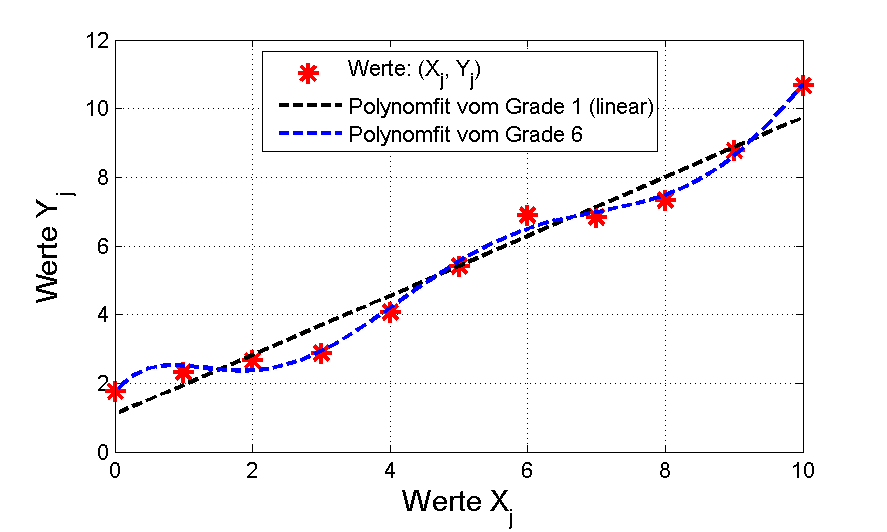
\includegraphics[width=11cm]{02_vorlesung/media/Regression_der_WertePaare.png}
    \caption{Beispiel für mögliche Fits, linearer Fit und Polynomfit vom Grade 6} \label{fig:LineareRegression}
\end{figure}
Bevor man mit der Regressionsrechnung anfängt, muss man sich im vorhinein sehr sorgfältig
überlegen, in welchem physikalischen Zusammenhang die Größen stehen, also welcher
Ansatz für das Messsystem als Modellgleichung sinnvoll ist.
In einigen Fällen ist dies auch eine Frage, welche Näherung für welchen Messbereich
ausreicht. 
% Abb.~\ref{fig:LineareRegression} illustriert die Abweichung der Wertepaare von den unterschiedlichen Modellen und damit wie gut verschiedene Modelle die Daten approximieren.

\textbf{Beispiel:} Bestimmung des Widerstandes $R$ durch lineare Regression \\
Wir erinnern uns wieder an das Beispiel aus der 1. Vorlesung (siehe z.~B. dort Abb.~1) und bestimmen den Ohmschen Widerstand $R$ sowie eine Offsetspannung $U_0$ bei gegebenen Werten einer
Präzisions\-strom\-quelle (Regressor, genau bekannt, d.h.\ keine Zufallsgröße) und beobachteten
Werten eines Voltmeters (Regressand, Zufallsgröße). 
Der Ohmsche Widerstand $R$ und die Offsetspannung $U_0$ sind die zu bestimmenden Modellparameter (Zufallsgrößen)

\begin{center}
	\begin{tabular}{l||c|c|c|c|c|c|c|c|c}
			\hline\hline
			$I$ in mA &    4.0 &     6.0 &     8.0 &    10.0 &    12.0 &    14.0 &    16.0 &    18.0 &    20.0\\
			\hline
			$U$ in mV &    62.5 &    51.5 &    96.0 &   140.2 &   138.9 &   195.1 &   225.8 &   207.8 &   223.7 \\
			\hline\hline
	\end{tabular}
\end{center}

Die Modellgleichung lautet mit den beiden Modellparametern 
$\theta_0 :=U_0$ und $\theta_1:=R$ 
\begin{equation}
U = U_0 + R \cdot I
\end{equation}

Die beiden Modellparameter können wir mit den beiden Gleichungen (siehe Gl. (\ref{eq:Lineare_Regressionskonstanten})) bestimmt werden.
\begin{equation}
\hat{U}_0 = \bar {U} - \hat{R} \bar {I} \quad \mathrm{und} \quad
\hat{R} = \frac{s_{IU} }{s_I^2 }
\label{eq:Lineare_Regressionskonstanten_Widerstand}
\end{equation}
Zunächst bestimmen wir die beiden Mittelwerte:
\begin{equation}
\bar{I}\; := \; \frac{1}{J} \, \sum\limits_{j = 1}^J \, I_j
= 12 \, \mathrm{mA}
\qquad 
\bar{U} \; := \; \frac{1}{J} \, \sum\limits_{j = 1}^J \, U_j
= 149.0556  \, \mathrm{mV}
\end{equation}
\begin{figure}
	\centering
	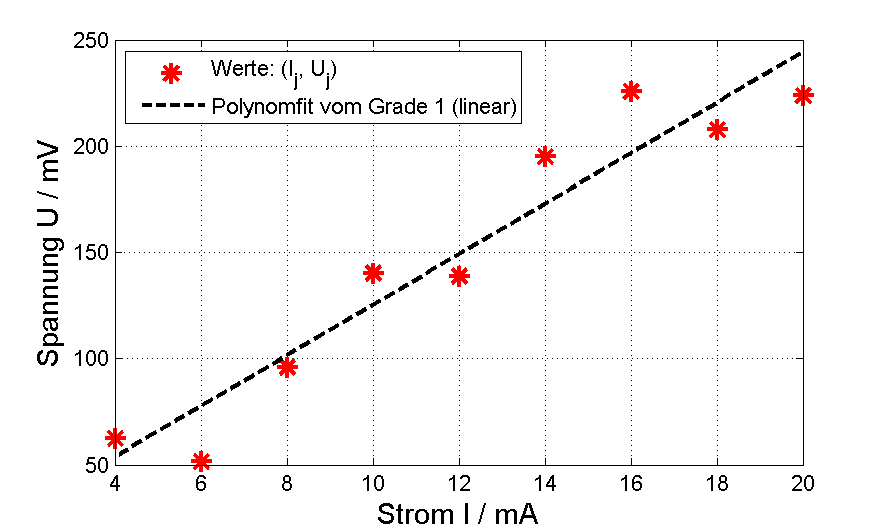
\includegraphics[width=11cm]{02_vorlesung/media/Regression_der_WertePaare_Strom_Spannung.png}
	\caption{Beispiel: Bestimmung des Ohmschen Widerstand und einer Offset-Spannung durch lineare Regression} \label{fig:LineareRegressionWiderstand}
\end{figure}
Die empirische Kovarianz mit den $J = 9$ Stichproben ergibt sich zu: 
\[
s_{IU} = \frac{1}{J - 1}\sum\limits_{j = 1}^J 
(I_j - \bar {R})(U_j - \bar {U}) = 357.0500  \, \mathrm{mA} \cdot \mathrm{mV}
\]

Die Varianz ergibt sich zu: 
\[
s_I^2 = \frac{1}{J - 1}\sum\limits_{j = 1}^J {(I_j - \bar {I})^2} = 30  \, \mathrm{mA}^2
\]

Somit erhalten wir als Schätzwert für $R$
\[
\hat{R} = \frac{s_{IU} }{s_I^2} = \frac{357.050 \, \mathrm{mA} \cdot \mathrm{mV}}{30 \, \mathrm{mA}^2} = 11.9017 
\, \frac{\mathrm{mV}}{\mathrm{mA}}
\]
mit $\frac{\mathrm{mV}}{\mathrm{mA}} = \frac{\mathrm{V}}{\mathrm{A}} = \mathrm{\Omega}$ also $\hat{R} = 11.9017 \, \mathrm{\Omega}$
und als Schätzwert für $U_0$: 
\[
\hat{U}_0 = \bar {U} - \hat{R} \bar {I} = 149.0556 \, \mathrm{mV}-  11.9017  \, \mathrm{\Omega} \cdot 12 \, \mathrm{mA} =
6.2356 \, \mathrm{mV}
\]

Das Ergebnis für die Regressionsgerade lautet somit
\begin{equation}
U = 6.2356  \, \mathrm{mV} + (11.9017 \, \mathrm{\Omega}) \cdot I 
\end{equation}
 und ist in Abb.~\ref*{fig:LineareRegressionWiderstand} dargestellt.

\section{Varianz der Regressionsparameter}
\label{subsec:vertrauensbereiche}
Es können aus den Messreihen die Varianzen der
geschätzten Regressionsparameter ermittelt werden. Das Verfahren zeigen wir
hier anhand der Regressionsgeraden mit den geschätzten Parametern
Achsenabschnitt $\hat{\theta}_0 $ und Steigung $\hat\theta_1 $.
Die Varianz der Schätzer liefert ein Ma{\ss} f\"{u}r die statistische
Sicherheit der Sch\"{a}tzung der Parameter $\theta _0 $ und
$\theta _1 $.
Für die Varianz des Regressionsparameters Steigung $\hat{\theta}_1 $
gilt:
\begin{equation}
\sigma^2_{\hat{\theta}_1} = \frac{ \hat \sigma^2_{\varepsilon}}{s^2_X \cdot (J- 1) }
\end{equation}
Für die Varianz des Regressionsparameters Achsenabschnitt $\hat{\theta}_0 $
gilt:
\begin{equation}
\sigma^2_{\hat{\theta}_0} = \hat \sigma^2_{\varepsilon} \cdot \left(\frac{1}{J}
	+ \frac{\bar {X}^2}{(J - 1) s_X^2 }\right)^2
\end{equation}
Die Varianz des Achsenabschnittes wird weiter unten in der Gl.(\ref{eq:Varianz des Achsenabschnitts}) hergeleitet. Dort ergibt sich \begin{equation}
\hat \sigma^2_{\theta_0}  = \hat \sigma^2_{\varepsilon}  \sum(X_j^2)  / (J \sum(X_j^2) - (\sum(X_j))^2) 
\end{equation}
Wir bezeichnen nun das $\hat \sigma^2_{\varepsilon}$ hier mit $s^2_{\varepsilon}$ und erhalten:
\begin{equation}
\hat \sigma^2_{\theta_0}  = s^2_{\varepsilon} \sum(X_j^2)  / (J \sum(X_j^2) - (\sum(X_j))^2) 
\end{equation}
\begin{equation}
\hat \sigma^2_{\theta_0} = s^2_{\varepsilon} \frac{1}{J} \sum(X_j^2)  / (\sum(X_j^2) - \frac{1}{J}(\sum(X_j))^2)
\end{equation}
Mit der folgenden Null-Identität
\begin{equation}
0 =  - \frac{1}{J}(\sum(X_j))^2 + \frac{1}{J}(\sum(X_j))^2
\end{equation}
gilt
\[
(1/J) \sum(X_j^2)  / (\sum(X_j^2) - \frac{1}{J}(\sum(X_j))^2) = 
\]
\[
(1/J) [\sum(X_j^2) - (1/J)(\sum(X_j))^2 + \frac{1}{J}(\sum(X_j))^2] / (\sum(X_j^2) - (1/J)(\sum(X_j))^2)
\]
das heisst
\[
\frac{1}{J} \sum(X_j^2)  / (\sum(X_j^2) - \frac{1}{J}(\sum(X_j))^2) =
\]
\[
(1/J) [ 1 + \frac{1}{J}(\sum(X_j))^2 / (\sum(X_j^2) - \frac{1}{J}(\sum(X_j))^2) ]
\]

und mit $(\sum(X_j^2) - \frac{1}{J}(\sum(X_j))^2) = (J-1) s_X^2$ gilt dann
\begin{align}
\hat \sigma^2_{\theta_0} =& 
s^2_{\varepsilon} \frac{1}{J} \sum(X_j^2)  / (\sum(X_j^2) - \frac{1}{J}(\sum(X_j))^2) \\
=& s^2_{\varepsilon} \frac{1}{J} \sum(X_j^2)  / (J-1) s_X^2
\end{align}
und mit der Umformung der Null-Identität gilt dann
\begin{align}
\hat \sigma^2_{\theta_0} 
=& s^2_{\varepsilon} \frac{1}{J} \sum(X_j^2)  / (\sum(X_j^2) - \frac{1}{J}(\sum(X_j))^2) \\
=& s^2_{\varepsilon} \frac{1}{J} \left[ 1 + \frac{1}{J}(\sum(X_j))^2 / (\sum(X_j^2) - \frac{1}{J}(\sum(X_j))^2) \right] \\
=& s^2_{\varepsilon} \frac{1}{J} \left[ 1 + \frac{1}{J(J-1) s_X^2} \left(\sum(X_j)\right)^2 \right]  
\end{align}
mit $\frac{1}{J}(\sum(X_j)) = \bar X$ gilt $\frac{1}{J}(\sum(X_j))^2 = J \bar X^2$
so dass
\begin{align}
\hat \sigma^2_{\theta_0} =& s_{\varepsilon} \frac{1}{J} \left[ 1 + 
\frac{1}{J (J-1) s_X^2} \left(\sum(X_j) \right)^2 \right] \\
=& s^2_{\varepsilon} \frac{1}{J(J-1) s_X^2} \left[ 1 + (J \bar X^2) \right] \\
=&
s^2_{\varepsilon}  \left[\frac{1}{J} + \frac{\bar X^2}{(J-1) s_X^2} \right]
\end{align}

Damit erhalten wir für die \textbf{Varianz bzw. die Unsicherheit des Achsenabschnittes}: 
\begin{equation}
\hat \sigma^2_{\theta_0} =
s^2_{\varepsilon}  \left[ \frac{1}{J} +\frac{\bar {X}^2}{(J - 1) s_X^2 } \right]
\end{equation}

\section{Matrixformalismus zur allgemeinen Lösung der linearen Regression}
\subsection{Matrixformalismus anhand der Regressionsgeraden}
Als Regressormatrix verwenden wir jetzt
\begin{equation}
\mathbf{X} \; = \;
\left(
\begin{array}{cc}
1 &  X_{1,1} \\
\vdots & \vdots\\
1 & X_{1,J} 
\end{array}
\right)
\end{equation}
Die Residuen berechnen sich wie folgt: 
\begin{equation}
\left(
\begin{array}{c}
\varepsilon_1\\
\vdots \\
\varepsilon_J
\end{array}
\right)  \; = \;
\left(
\begin{array}{c}
Y_{1} \; - \; (1 \, \theta_0 \; + \;  X_{1,1} \, \theta_1)\\
\vdots \\
Y_{J} \; - \; (1 \, \theta_0 \; + \;  X_{1,J} \, \theta_1)
\end{array}
\right) \; = \;
\left(
\begin{array}{c}
Y_{1}\\
\vdots \\
Y_{J}
\end{array}
\right) 
\; - \; 
\left(
\begin{array}{cc}
1 &  X_{1,1} \\
\vdots & \vdots\\
1 & X_{1,J} 
\end{array}
\right) 
\left(
\begin{array}{c}
\theta_0\\
\theta_1
\end{array}
\right)
\label{linearRegressionGeradeTheta}
\end{equation}
Die Summe der Quadrate der Residuen $\sum_{j=1}^J \varepsilon_j^2$ lässt sich ebenso
mit der Rechenregel Zeile mal Spalte schreiben, als Zeilenvektor mal Spaltenvektor
\begin{equation}
\sum_{j=1}^J \varepsilon_j^2 \; = \; 
\left(\begin{array}{ccc}
\varepsilon_1 & \dots & \varepsilon_J
\end{array}
\right)
\left(
\begin{array}{c}
\varepsilon_1\\
\vdots \\
\varepsilon_J
\end{array}
\right)
\end{equation}
Dabei heißt der Zeilenvektor der transponierte Vektor, also
\begin{equation}
\boldsymbol{\varepsilon}^\mathsf{T} \; = \; \left(\begin{array}{ccc}
\varepsilon_1 & \dots & \varepsilon_J
\end{array}
\right) \qquad \mathrm{und}  \qquad 
\boldsymbol{\varepsilon} \; = \; \left(
\begin{array}{c}
\varepsilon_1\\
\vdots \\
\varepsilon_J
\end{array}
\right)
\end{equation}
und ferner führen wir ein
\begin{equation}
\boldsymbol{\theta} \; = \;
\left(
\begin{array}{c}
\theta_0\\
\theta_1
\end{array}
\right) \qquad \mathrm{und}  \qquad 
\mathbf{Y}  \; = \;\left(
\begin{array}{c}
Y_{1}\\
\vdots \\
Y_{J}
\end{array}
\right) 
\end{equation}
und Gl.~(\ref{linearRegressionGeradeTheta}) sieht in transponierter Schreibweise
wie folgt aus
\begin{equation}
\boldsymbol{\varepsilon}^\mathsf{T} \; = \;
\mathbf{Y}^\mathsf{T}
\; - \; 
\boldsymbol{\theta}^\mathsf{T} \left(
\begin{array}{cc}
1 &  X_{1,1} \\
\vdots & \vdots\\
1 & X_{1,J} 
\end{array}
\right)^\mathsf{T} 
\label{linearRegressionGeradeTransponiert}
\end{equation}
d.h.
\begin{equation}
\boldsymbol{\varepsilon}^\mathsf{T} \; = \;
\mathbf{Y}^\mathsf{T}
\; - \; 
\left(
\begin{array}{cc}
\theta_0 &
\theta_1
\end{array}
\right) \left(
\begin{array}{ccc}
1 &  \dots & 1 \\
X_{1,1} & \dots & X_{1,J} 
\end{array}
\right).
\label{linearRegressionGeradeUmform}
\end{equation}
Die Summe der Quadrate der Residuen $\sum_{j=1}^J \varepsilon_j^2$  sieht damit wie
folgt aus
\begin{equation}
\boldsymbol{\varepsilon}^\mathsf{T}  \boldsymbol{\varepsilon} \; = \;
\left(
\mathbf{Y}^\mathsf{T}
\; - \; 
\boldsymbol{\theta}^\mathsf{T} \mathbf{X}^\mathsf{T} \right)
\left(
\mathbf{Y}
\; - \; 
\mathbf{X} \boldsymbol{\theta} \right)
\end{equation}
d.h.
\begin{equation}
\boldsymbol{\varepsilon}^\mathsf{T}  \boldsymbol{\varepsilon} \; = \;
\mathbf{Y}^\mathsf{T} \mathbf{Y}
\; - \; 
\boldsymbol{\theta}^\mathsf{T} \mathbf{X}^\mathsf{T}  \mathbf{Y} 
\; - \; 
\mathbf{Y}^\mathsf{T}  \mathbf{X} \boldsymbol{\theta}
\; + \; 
\boldsymbol{\theta}^\mathsf{T} \mathbf{X}^\mathsf{T} \mathbf{X} \boldsymbol{\theta}
\end{equation}
Für die Ableitungen nach den $\theta_0, \theta_1$ gilt
\begin{equation}
\frac{\partial}{\partial \theta_l} \sum_{j=1}^J \varepsilon_j^2 \; = \; 
2 \sum_{j=1}^J \varepsilon_j \frac{\partial}{\partial \theta_l} \varepsilon_j \; = \; 
2 \sum_{j=1}^J \varepsilon_j (-1) \frac{\partial}{\partial \theta_l}(1 \, \theta_1 \; + \;  X_{1,j} \, \theta_2) \; = \; 0
\end{equation}
wobei $l = 0,1$ ist also
\begin{equation}
\sum_{j=1}^J \varepsilon_j  \frac{\partial}{\partial \theta_0}(1 \, \theta_0 \; + \;  X_{1,j} \, \theta_1)  \; = \; 0 \qquad \mathrm{und} \qquad 
\sum_{j=1}^J \varepsilon_j  \frac{\partial}{\partial \theta_1}(1 \, \theta_0 \; + \;  X_{1,j} \, \theta_1)  \; = \; 0
\end{equation}
also
\begin{equation}
\sum_{j=1}^J \varepsilon_j (1) \; = \; 0 \qquad \mathrm{und}  \qquad 
\sum_{j=1}^J \varepsilon_j ( X_{1,j})  \; = \; 0
\end{equation}
Dies sieht in Matrixschreibweise als $2 \times 2$-Gleichungssystem wie folgt aus
\begin{equation}
\boldsymbol{\varepsilon}^\mathsf{T} \, \mathbf{X} \; = \;
\left(
\begin{array}{c}
0\\
0
\end{array}
\right)
\end{equation}
d.h.
\begin{equation}
\left(\mathbf{Y}^\mathsf{T}
\; - \; 
\boldsymbol{\theta}^\mathsf{T} \mathbf{X}^\mathsf{T} \right) \, \mathbf{X} \; = \;
\left(
\begin{array}{c}
0\\
0
\end{array}
\right)
\end{equation}
d.h.
\begin{equation}
\boldsymbol{\theta}^\mathsf{T} \, \mathbf{X}^\mathsf{T}  \, \mathbf{X} \; = \;
\mathbf{Y}^\mathsf{T} \, \mathbf{X}
\end{equation}
%$\frac{\partial}{\partial \beta_l} \varepsilon_j$ auf.
%Der Vektor mit für die partielle Differentiation heißt Nablaoperator
%\begin{equation}
%\nabla_\beta \; = \;
%\left(
%\begin{array}{cc}
%\frac{\partial}{\partial \beta_0} &
%\frac{\partial}{\partial \beta_1}
%\end{array}
%\right)
%\end{equation}
das ist äquivalent zu
\begin{equation}
\mathbf{X}^\mathsf{T} \, \mathbf{X} \, \boldsymbol{\theta} \; = \;
\mathbf{X}^\mathsf{T} \, \mathbf{Y} .
\end{equation}
Die numerische Lösung des Gleichungssystems liefert dann die Schätzwerte zu
den Regressionparametern $\boldsymbol{\theta}$. Ein mögliches Verfahren zum
Lösen des linearen Gleichungssystems ist das Gauß-Jordan-Eliminationsverfahren, zu
dem im Anhang dieses Skripts der Quellcode gemäß den \textsl{Numerical Recipes}
\cite{Fla02} abgedruckt ist.
Formal notieren wir 
die Schätzer (als solche kenntlich durch das Dach) wie folgt
\begin{equation}
\boldsymbol{\hat \theta} \; = \;
\left( \mathbf{X}^\mathsf{T}  \, \mathbf{X} \right)^{-1} \mathbf{X}^\mathsf{T} \, \mathbf{Y}
\end{equation}
wobei hoch minus Eins soviel bedeutet wie die Inverse der Matrix.

Als nächstes ermitteln wir, um das \textbf{vollständige
	Messergebnis} zu erhalten, auch die Schätz\-werte der Kovarianzen. Die
Hauptdiagonale der Kovarianzmatrix sind die Varianzen.
\begin{equation}
\operatorname {Cov}( \boldsymbol{\theta},\boldsymbol{\theta} ) \; = \;
\operatorname {Cov} 
\left(\left( \mathbf{X}^\mathsf{T}  \, \mathbf{X} \right)^{-1} \mathbf{X}^\mathsf{T} \, \mathbf{Y}, \left( \mathbf{X}^\mathsf{T}  \, \mathbf{X} \right)^{-1} \mathbf{X}^\mathsf{T} \, \mathbf{Y}\right)
\end{equation}
%mit Gl.~(\ref{CovarianzKonstMatrix}) ist dies
das ist
\begin{equation}
\operatorname {Cov}( \boldsymbol{\theta}, \boldsymbol{\theta} ) \; = \;
\left( \mathbf{X}^\mathsf{T}  \, \mathbf{X} \right)^{-1} \mathbf{X}^\mathsf{T} \operatorname {Cov} (\mathbf{Y}, \mathbf{Y}) \, \left( \left( \mathbf{X}^\mathsf{T}  \, \mathbf{X} \right)^{-1} \mathbf{X}^\mathsf{T} \right)^\mathsf{T}
\end{equation}
und mit Einsetzen der aus den Schätzern $\boldsymbol{\hat \theta}$ erhaltenen
empirischen Varianz der Residuen 
$\operatorname {Cov} (\mathbf{Y}, \mathbf{Y}) = \operatorname {Var} (\mathbf{\varepsilon}) = \hat \sigma_{\varepsilon}^2$
bekommen wir die empirische Kovarianzmatrix
\begin{equation}
\boldsymbol{\hat \Sigma}_{\boldsymbol{\theta}} \; = \;
\hat \sigma_{\varepsilon}^2
\left( \mathbf{X}^\mathsf{T}  \, \mathbf{X} \right)^{-1} \mathbf{X}^\mathsf{T} \, \left( \left( \mathbf{X}^\mathsf{T}  \, \mathbf{X} \right)^{-1} \mathbf{X}^\mathsf{T} \right)^\mathsf{T}
\end{equation}
mit
$$
\operatorname {Var} (\mathbf{\varepsilon}) = \hat \sigma_{\varepsilon}^2 \; = \;
\frac{1}{J-M} \, \boldsymbol{\hat \varepsilon}^\mathsf{T} \boldsymbol{\hat \varepsilon}
$$
wobei $M$ die Anzahl der Regressionsparameter ist, also $M = 2$ im Fall der Geraden, für die beiden Parameter Achsenabschnitt und Steigung und
$$
\boldsymbol{\hat \varepsilon} \; = \; \mathbf{Y} \, - \, \mathbf{X} \boldsymbol{\hat \theta} .
$$

Ferner gilt mit $\left( \left( \mathbf{X}^\mathsf{T}  \, \mathbf{X} \right)^{-1} \mathbf{X}^\mathsf{T} \right)^\mathsf{T} = \mathbf{X} \left( \mathbf{X}^\mathsf{T}  \, \mathbf{X} \right)^{-1}$
\begin{equation}
\boldsymbol{\hat \Sigma}_{\boldsymbol{\theta}} \; = \; \hat \sigma_{\varepsilon}^2
\left( \mathbf{X}^\mathsf{T}  \, \mathbf{X} \right)^{-1} \mathbf{X}^\mathsf{T}  \,  \mathbf{X} \, \left( \mathbf{X}^\mathsf{T}  \, \mathbf{X} \right)^{-1} 
\end{equation}
und mit $\left( \mathbf{X}^\mathsf{T}  \, \mathbf{X} \right)^{-1} \mathbf{X}^\mathsf{T}  \, \mathbf{X}  \; = \; 1 \! \mathrm{I}$ Einheitsmatrix
\begin{equation}
\boldsymbol{\hat \Sigma}_{\boldsymbol{\theta}} \; = \; \hat \sigma_{\varepsilon}^2
\left( \mathbf{X}^\mathsf{T}  \, \mathbf{X} \right)^{-1}
\label{UnsicherheitRegressparams}
\end{equation}
Gleichung (\ref{UnsicherheitRegressparams}) liefert die Unsicherheit für die Regressionsparameter
$\boldsymbol{\theta}$. 
%Sie unterscheidet sich
%Gleichung (\ref{KovarianzSumme})
Setzen wir dies nun für die Regressionsgerade ein, also setzen wir
$$
\mathbf{X} \; = \;
\left(
\begin{array}{cc}
1 &  X_{1,1} \\
\vdots & \vdots\\
1 & X_{1,J} 
\end{array}
\right)
$$
ein, so erhalten wir für
\begin{equation}
\left( \mathbf{X}^\mathsf{T}  \, \mathbf{X} \right)^{-1} \; = \;
\left( \left(
\begin{array}{ccc}
1 & \cdots & 1 \\
X_{1,1} & \cdots & X_{1,J} 
\end{array}
\right)
\, 
\left(
\begin{array}{cc}
1 &  X_{1,1} \\
\vdots & \vdots\\
1 & X_{1,J} 
\end{array}
\right) \right)^{-1}
\end{equation}
d.h.
\begin{equation}
\left( \mathbf{X}^\mathsf{T}  \, \mathbf{X} \right)^{-1} \; = \;
\left(
\begin{array}{ccc}
J & \sum\limits_{j=1}^J X_{1,j} \\
\sum\limits_{j=1}^J X_{1,j} & \sum\limits_{j=1}^J X_{1,j}^2
\end{array}
\right)^{-1}
\end{equation}
d.h.
\begin{equation}
\left( \mathbf{X}^\mathsf{T}  \, \mathbf{X} \right)^{-1} \; = \;
\frac{1}{J \, \sum\limits_{j=1}^J X_{1,j}^2 \; - \;
	\left(\sum\limits_{j=1}^J X_{1,j}\right)^2}
\left(
\begin{array}{ccc}
\sum\limits_{j=1}^J X_{1,j}^2 & -\sum\limits_{j=1}^J X_{1,j} \\
-\sum\limits_{j=1}^J X_{1,j} & J
\end{array}
\right)
\end{equation}
so dass wir für den Achsenabschnitt $\theta_0$ und die Steigung $\theta_1$ folgende
empirische Varianzen und Kovarianzen erhalten
\begin{equation}
\left(\begin{array}{cc}
\hat \sigma^2_{\theta_0} &\hat \sigma_{\theta_0, \theta_1}\\
\hat \sigma_{\theta_0, \theta_1} & \hat \sigma^2_{\theta_1} 
\end{array}\right)
\; = \;
\frac{\hat \sigma^2_\varepsilon}{J \, \sum\limits_{j=1}^J X_{1,j}^2 \; - \; 
	\left(\sum\limits_{j=1}^J X_{1,j}\right)^2}
\left(
\begin{array}{ccc}
\sum\limits_{j=1}^J X_{1,j}^2 & -\sum\limits_{j=1}^J X_{1,j} \\
-\sum\limits_{j=1}^J X_{1,j} & J
\end{array}
\right)
\end{equation}
oder einzeln aufgeschrieben, die Varianz des Achsenabschnitts
%\begin{figure}
%	\begin{center}
%		\includegraphics[width=100mm]{Bilder/regressionNormalResi_Perr_1a.eps}
%		\caption{\label{regressionParamErr} Unsicherheit der Schätzer
%			der linearen Regression einer Geradengleichung für ein
%			Vertrauensniveau von $98 \%$. Mit $\nu = J-2 = 26-2 = 24$ Freiheitsgraden
%			ist das Quantil der Student-t-Verteilung $t_{1-\alpha/2,\nu} = 2.492$.}
%	\end{center}
%\end{figure}
\begin{equation}
\hat \sigma^2_{\theta_0} \; = \; 
\frac{\hat \sigma^2_\varepsilon \, \sum\limits_{j=1}^J X_{1,j}^2}{J \, 
	\sum\limits_{j=1}^J X_{1,j}^2 \; - \; \left(\sum\limits_{j=1}^J X_{1,j}\right)^2}
\label{eq:Varianz des Achsenabschnitts}
\end{equation}
die Kovarianz für Achsenabschnitt und Steigung
\begin{equation}
\hat \sigma_{\theta_0, \theta_1} \; = \; 
\frac{- \hat \sigma^2_\varepsilon \, \sum\limits_{j=1}^J X_{1,j}}{J \, \sum_{j=1}^J X_{1,j}^2 \;
	- \; \left(\sum\limits_{j=1}^J X_{1,j}\right)^2}
\end{equation}
und die Varianz der Steigung
\begin{equation}
\hat \sigma^2_{\theta_1} \; = \; 
\frac{\hat \sigma^2_\varepsilon}{\sum\limits_{j=1}^J X_{1,j}^2 \; - \; 
	\frac{1}{J}\left(\sum\limits_{j=1}^J X_{1,j}\right)^2} .
\end{equation}
Die Standardabweichungen zu jedem Regressionsparameter $\theta_l$ mit $l = 0,\dots,M-1$ sind
die Wurzel aus den Varianzen, die auf der Hauptdiagonalen der Kovarianzmatrix 
$\left( \mathbf{X}^\mathsf{T}  \, \mathbf{X} \right)^{-1} \, \hat \sigma_{\varepsilon}^2$
stehen. In der üblichen englischsprachigen Literatur zur Regressionrechnung wird
die Standardabweichung der Regressionsparameter \textsl{Standard Error} genannt.
\subsection{Matrixansatz als allgemeiner Ansatz für linearen Regression}
Die behandelten allgemeinen Formen von Problemstellungen zur Schätzung von Modellparametern
werden wir in dieser Vorlesungsreihe nicht weiter vertiefen. Sie sollen lediglich einen Einblick
und Überblick über die vielfältigen Möglichkeiten in diesem Bereich liefern.
In den Übungen und der Klausur werden
wir uns auf das Schätzverfahren mittels linearer Regression fokussieren.


Um die lineare Regression universeller einsetzen zu können, ob nun Polynome oder
Ebenen oder Paraboloide zu fitten sind, ist es erforderlich den allgemeinen Ansatz zu verstehen
und die unterschiedlichen Anwendungen so formulieren zu können, dass sie darüber lösbar werden.

Wir wollen also den Übergang von Gl.~(\ref{linearRegressionGeradeTheta}) mit
\begin{equation*}
\left(
\begin{array}{c}
\varepsilon_1\\
\vdots \\
\varepsilon_J
\end{array}
\right)  \; = \;
\left(
\begin{array}{c}
 Y_{1} \; - \; (1 \, \theta_0 \; + \;  X_{1,1} \, \theta_1)\\
\vdots \\
 Y_{J} \; - \; (1 \, \theta_0 \; + \;  X_{1,J} \, \theta_1)
\end{array}
\right) \; = \;
\left(
\begin{array}{c}
 Y_{1}\\
\vdots \\
 Y_{J}
\end{array}
\right) 
\; - \; 
\left(
\begin{array}{cc}
 1 &  X_{1,1} \\
\vdots & \vdots\\
 1 & X_{1,J} 
\end{array}
\right) 
\left(
\begin{array}{c}
\theta_0\\
\theta_1
\end{array}
\right)
\end{equation*}
mit
\begin{equation*}
\mathbf{X} \; = \;
\left(
\begin{array}{cc}
 1 &  X_{1,1} \\
\vdots & \vdots\\
 1 & X_{1,J} 
\end{array}
\right)
\end{equation*}
zu einer allgemeinen Formulierung finden.

Für $M$ Regressoren wird die Regressormatrix zu einer $J \times M$-Matrix, also einer Matrix
aus $M$ Spalten und $J$ Zeilen aufgestellt:
\begin{equation}
\mathbf{X} \; = \;
\left(
\begin{array}{ccc}
 X_{1,1} & \dots &  X_{M,1} \\
\vdots & & \vdots \\
 X_{1,J}  & \dots &  X_{M,J}
\end{array}
\right)
\end{equation}
Die Indexschreibweise ist hier relativ zur Schreibweise der Matrizenrechnung vertauscht, weil wir den Index für die
Messgrößen vorne haben gefolgt von dem Index für die Beobachtungen, wir aber die Messgrößen als
Spaltenvektoren verwenden und somit den Index für die Beobachtungen als Zeilenindex haben.

\begin{equation}
\boldsymbol{\varepsilon} \, =  \, \left(
\begin{array}{c}
\varepsilon_1\\
\vdots \\
\varepsilon_J
\end{array}
\right)  \; = \;
\left(
\begin{array}{c}
 Y_{1} \; - \; (X_{1,1} \, \theta_1  \; + \; \dots  \; + \;  X_{M,1} \, \theta_{M})\\
\vdots \\
 Y_{J} \; - \; (X_{1,J} \, \theta_1 \; + \; \dots  \; + \;  X_{M,J} \, \theta_{M})
\end{array}\right)  \, = \, 
\mathbf{Y} \, -  \, \mathbf{X} \, \boldsymbol{\theta}
\end{equation}
Im Fall eines Polynoms kann jeder der Regressoren Funktion derselben Messgröße sein.
Dies kann beispielsweise einfach
durch folgenden Potenzansatz $X_{m,j} = X_{1,j}^{m-1}$ mit $m = 1,\dots,M$ als
Polynom vom Grad $M-1$ dargestellt werden
\begin{equation}
\left(
\begin{array}{c}
\varepsilon_1\\
\vdots \\
\varepsilon_J
\end{array}
\right)  \; = \;
\left(
\begin{array}{c}
 Y_{1} \; - \; (X_{1,1}^0 \, \theta_1  \; + \; \dots  \; + \;  X_{1,1}^{M-1} \, \theta_{M})\\
\vdots \\
 Y_{J} \; - \; (X_{1,J}^0 \, \theta_1 \; + \; \dots  \; + \;  X_{1,J}^{M-1} \, \theta_{M})
\end{array}\right)
\end{equation}
wobei $X_{1,j}^0 = 1$ ist.

Wird die Regressormatrix zu Beginn korrekt aufgestellt, so lassen sich die 
$M$ Regressionsparameter $\boldsymbol{\theta}$
schätzen durch numerische Lösung des folgenden Gleichungssystems:
\begin{equation}
\mathbf{X}^\mathsf{T} \, \mathbf{X} \, \boldsymbol{\theta} \; = \;
\mathbf{X}^\mathsf{T} \, \mathbf{Y} .
\label{LsgRegressionGlSys}
\end{equation}
Dass nach Lösen des Gleichungssystems Schätzwerte für
die Parameter gewonnen wurden, wird durch das Dach auf dem Symbol $\boldsymbol{\theta}$ gekennzeichnet.
\begin{equation}
 \boldsymbol{\hat \theta} \; = \;
\left( \mathbf{X}^\mathsf{T}  \, \mathbf{X} \right)^{-1} \mathbf{X}^\mathsf{T} \, \mathbf{Y}
\label{eq:schaetzwerte_fuer_theta}
\end{equation}
wobei hoch minus Eins soviel bedeutet wie die Inverse der Matrix.
Für Varianzen und Kovarianzen der $M$ Regressionsparameter $\theta_1, \dots, \theta_M$
werden die Residuen gebraucht
\begin{equation}
\boldsymbol{\hat \varepsilon} \, =  \, \left(
\begin{array}{c}
\hat \varepsilon_1\\
\vdots \\
\hat \varepsilon_J
\end{array}
\right)  \; = \;
\left(
\begin{array}{c}
 Y_{1} \; - \; (X_{1,1} \, \hat \theta_1  \; + \; \dots  \; + \;  X_{M,1} \, \hat \theta_{M})\\
\vdots \\
 Y_{J} \; - \; (X_{1,J} \, \hat \theta_1 \; + \; \dots  \; + \;  X_{M,J} \, \hat \theta_{M})
\end{array}
\right) \, = \, 
\mathbf{Y} \, -  \, \mathbf{X} \, \boldsymbol{\hat \theta}
\end{equation}
um deren empirische Varianz zu berechnen
\begin{equation}
\hat \sigma_{\varepsilon}^2 \; = \;
\frac{1}{J-M} \, \boldsymbol{\hat \varepsilon}^\mathsf{T} \boldsymbol{\hat \varepsilon}
\end{equation}
so dass wir die empirische Kovarianzmatrix der Parameter gmäß Gl.~(\ref{UnsicherheitRegressparams}) erhalten:
\begin{equation*}
\boldsymbol{\hat \Sigma}_{\boldsymbol{\theta}} \; = \; 
\left( \mathbf{X}^\mathsf{T}  \, \mathbf{X} \right)^{-1} \;
\hat \sigma_{\varepsilon}^2
\end{equation*}
Um die Unsicherheit der einzelnen Regressionsparameter zu erhalten, führen wir Einheitsvektoren ein, die $M$-dimensional sind.
Bei dem $l$-ten Einheitsvektor sind die ersten $l-1$ Vektorkomponenten Nullen, an der $l$-ten Stelle steht eine Eins
und die $l+1$-te Komponente bis zur $M$-ten sind wieder Nullen.
\begin{equation}
\boldsymbol{e}_l \; = \;
\left(\begin{array}{c}
0\\
\vdots\\
0\\
1\\
0\\
\vdots\\
0
\end{array}\right)
\end{equation}
Dann lässt sich durch folgende Multiplikation die $l$-te Varianz, d.h. das $l$-te Element
der Hautpdiagonalen aus der Kovarianzmatrix herausholen
\begin{equation}
\hat \sigma_l^2 \; = \; \boldsymbol{e}_l^\mathsf{T} \, \left( \mathbf{X}^\mathsf{T}  \, \mathbf{X} \right)^{-1} \, \boldsymbol{e}_l  \; \hat \sigma_{\varepsilon}^2 .
\end{equation}
Die Standardabweichung (\textsl{Standard Error}) wird daraus durch Ziehen der Wurzel
gewonnen
\begin{equation}
\hat \sigma_l \; = \; \sqrt{\hat \sigma_l^2} .
\end{equation}
Im fünften Kapitel werden wir dann sehen, wie man mit Hilfe der Varianzen bzw. Standardabweichungen Vertrauensintervalle für die geschätzten Modellparameter bestimmt.
Die Herleitung ist im Anhang aufgeschrieben.

\newpage
\section{Das Bestimmtheitsmaß, empirischer Korrelationskoeffizient}
Die G\"{u}te des gew\"{a}hlten linearen Ansatzes kann mit dem
\textbf{Bestimmtheitsmaß} $\rho_{XY}^2 $ bzw. dem \textbf{empirischen
	Korrelationskoeffizienten} $\rho_{XY}$ beurteilt werden, aber nur dann
wenn ein solcher Zusammenhang auch existiert. Der empirische
Korrelationskoeffizienten gibt den Grad der linearen
Abh\"{a}ngigkeit zwischen den Messwerten $(X_1 ,\ldots ,X_J )$ und
$(Y_1 ,\ldots ,Y_J)$ an. 

Für den empirischen Korrelationskoeffizienten $\rho_{XY}$ gilt folgendes:

\begin{center}
	\begin{tabular}
		{|p{100pt}|p{209pt}|} \hline 
		$\rho_{XY} = \pm 1$&
		100{\%} lineare Abh\"{a}ngigkeit  \\
		\hline $\rho_{XY} = 0$&
		keine lineare Abh\"{a}ngigkeit \\
		\hline $\rho_{XY} > \mbox{bzw.} < 0$&
		gleich-/gegenl\"{a}ufige lineare Abh\"{a}ngigkeit \\
		\hline
	\end{tabular}
\end{center}

F\"{u}r die Bestimmung des Bestimmtheitsma{\ss}es oder des
empirischen Korrelationskoeffizient f\"{u}hrt man eine Streuungs-
bzw. Varianzanalyse durch. Man kann bei der linearen Regression 3
Arten von Streuungen unterscheiden:
\begin{itemize}
	\item[] $s_{\mathrm{T}}^2:$~die \textbf{totale empirische Varianz}
	\item[] $s_{\mathrm{M}}^2:$~die \textbf{empirische Varianz auf Grund des Modells}
	\item[] $s_{\mathrm{R}}^2:$~die \textbf{restliche empirische Varianz}
\end{itemize}
Die totale Streuung ist bei unabhängigen direkten Messgrößen $X_j$ gegeben
durch:
\begin{equation}
s_{\mathrm{T}}^2 = \frac{1}{J - 1}\sum\limits_{j = 1}^J {(Y_j - \bar {Y})^2}
\quad \mathrm{mit~} Y_j : \mathrm{Messwert ~zu~}  X_j 
\end{equation}
Die empirische Varianz auf Grund des Modells beschreibt die
Streuung der Y-Werte auf der Regressionsgeraden in Bezug zum
Mittelwert $\bar{Y}$, d.~h.
\begin{equation}
s_{\mathrm{M}}^2 = \frac{1}{J - 1}\sum\limits_{j = 1}^n {(\hat{\theta}_0 + \hat{\theta}_1 X_j - \bar
	{Y})^2}
\end{equation}
Die Differenz zwischen $Y_j$ und $\hat{\theta}_0 + \hat{\theta}_1 X_j $ bleiben im
Modell unerkl\"{a}rt, sie wird als restliche Streuung bezeichnet:
\begin{equation}
s_{\mathrm{R}}^2 = \frac{1}{J - 1}\sum\limits_{j = 1}^J {(Y_j - (\hat{\theta}_0 
	+ \hat{\theta}_1 X_j))^2}
\end{equation}
Man kann nun folgendes Bemerkenswerte zeigen:
\begin{equation}
s_{\mathrm{T}}^2 = s_{\mathrm{M}}^2 + s_{\mathrm{R}}^2
\end{equation}
Das Bestimmtheitsma{\ss} ist definiert als das Verh\"{a}ltnis von
empirischer Varianz des Modells zu der totalen Varianz:
\[
\rho_{XY}^2 = \frac{s_{\mathrm{M}}^2}{s_{\mathrm{T}}^2} = \frac{\sum\limits_{j = 1}^J {(\hat{\theta}_0 + \hat{\theta}_1 X_j - \bar {Y})^2} }{\sum\limits_{j = 1}^J {(Y_j - \bar{Y})^2} }
\]
Mit dem Schwerpunkt $\bar {Y} = \hat{\theta}_0 + \hat{\theta}_1 \bar {X}$ ergibt sich:
\[
\rho_{XY}^2 = \frac{\hat{\theta}_1^2 \cdot \sum\limits_{j = 1}^J 
	{(X_j - \bar X)^2} }{\sum\limits_{j = 1}^J {(Y_j - \bar {Y})^2} }
\]
Mit den Regressionsparametern $\hat{\theta}_1 = \frac{\sum\limits_{j =
		1}^J {(X_j - \bar {X})(Y_j - \bar {Y})} }{\sum\limits_{j = 1}^J {(X_j
		- \bar {X})^2} }$ (siehe Gl.(\ref{eq:Lineare_Regressionskonstanten})) erhält man für das 
Bestimmtheitsmaß:
\begin{align}
\rho_{XY}^2 &= \frac{\left[ {\sum\limits_{j = 1}^J {(X_j - \bar {X})(Y_j - \bar{Y})} } \right]^2}{\sum\limits_{j = 1}^J {(X_j - \bar {X})^2}
	\cdot
	\sum\limits_{j = 1}^J {(Y_j - \bar {Y})^2} } \nonumber \\[2ex]
&= \frac{s_{XY} ^2}{s_X ^2 \cdot s_Y ^2} \quad \textrm{mit}\; 
0 \le \rho_{XY}^2 \le 1 
\end{align} 
Den empirischen Korrelationskoeffizienten kann man somit wie folgt
berechnen:
\begin{equation}
\rho_{XY} = \frac{ s_{XY} }{ s_X \cdot s_Y } \quad \mathrm{~mit~}  - 1 \le \rho_{XY} \le 1
\end{equation}
\newpage
\section{Beispiele zur Linearen Regression}
\label{Vorl2Regressionsaufg2}
\subsection{Fit einer Geraden}
Gegeben sind 5 Messpunkte
\begin{table}[htb!]
	\centering
	\begin{tabular}{l|c c c c c c}
		$X_i$ & 1 & 2 & 3 & 4 & 5 \\ \hline
		$Y_i$ & 0.4 & 0.55 & 0.70 & 0.75 & 0.8
	\end{tabular}
\end{table}
\begin{itemize}
	\item [(a)] Führen Sie eine lineare Regression durch, indem
	Sie den y-Abschnitt $\hat\theta_0$ und die Steigung $\hat\theta_1$ bestimmen. Geben Sie das Bestimmtheitsmaß $\rho_{XY}^2$ an.
	\item[(b)] Bestimmen Sie die Residuen $\varepsilon_j$ und das 
	Qualitätsmaß $Q(\hat\theta _0,\hat\theta _1)$ der Regression. Geben Sie die Varianz der Residuen 
	$s^2(\hat\theta_0,\hat{\theta_1})$ an?
	\item[(c)] Geben Sie den Standardabweichung (standard error) der beiden 
	Regressionsparameter $\hat\theta_0$ und $\hat\theta_1$ an?
	
	% Geben Sie das 95\%ige Vertrauensintervall
	% von	$\hat\theta_0$ und $\hat\theta_1$ an.
	% 	Es wird dazu das t-Quantil für 3 Freiheitsgrade (5 Messpunkte minus
	%	2 Parameter = 3 Freiheitsgrade) benötigt.
	%	Das t-Quantil für den beidseitigen Vertrauensbereich von 95\%
	%	für 3 Freiheitsgrade ist gegeben durch $t_3=3.1824$. 
	%		\newline
	%	Man erhält das t-Quantil durch den Matlab/Octave-Befehl: \texttt{tinv(0.975,3) = 3.31824} (\texttt{tinv} berechnet den einseitigen Vertrauensbereich)
	%	oder man schlägt in einem Tabellenwerk nach;
	%	siehe z.~B. https://de.wikipedia.org/wiki/Studentsche\_t-Verteilung
\end{itemize}

Mit der Gl.(\ref{eq:schaetzwerte_fuer_theta}) können wir 
das Beispiel lösen. Der Matlab/Octave-Code lautet: 
\begin{verbatim}
close all; clear all;
% Eingabe der Messwertepaare
input = [...                 
1, 0.4;...                
2, 0.55;...
3, 0.7;...
4, 0.75; ...
5, 0.8];
m = length(input);             % Anzahl der Messpunkte
X = [ones(m,1), input(:,1)];   % Aufstellen der X-Matrix
Y = input(:,2);                % Aufstellen der Y-Matrix
% degree of freedom 
df = 5-2;
% Berechung der Schätzwerte \thetaHat; 
% y-Abschnitt = \thetaHat(1); Steigung = \thetaHat(2)
thetaHat = (X' * X) \ (X' * Y);    
% Anzeige der Schätzwerte
disp(thetaHat);
% Plotten der Regressionsgeraden
xx = linspace(0,6,100);
yy = thetaHat(1) + thetaHat(2)*xx;
figure(10)
plot(xx, yy,'linewidth',1.5)
% Plotten der Datenwerte 
hold on
plot(input(:,1), input(:,2), 'or','linewidth',2, 'MarkerSize',6)
hold off
grid on; 
xlabel('Werte X_j','fontsize',14)
ylabel('Werte Y_j','fontsize',14)
set(gcf, 'PaperUnits', 'centimeters');
x_width=15 ;y_width= 9;
set(gcf, 'PaperPosition', [0 0 x_width y_width]);
print '-dpng' LinRegression.png
\end{verbatim}

Als Lösung erhalten wir den Plot in Abb.\ref{fig:LineareRegression}.
Der y-Achsenabschnitt liegt bei 0.34 und die Steigung ist 0.1.
\begin{figure}[!htp]
	\begin{center}
		%		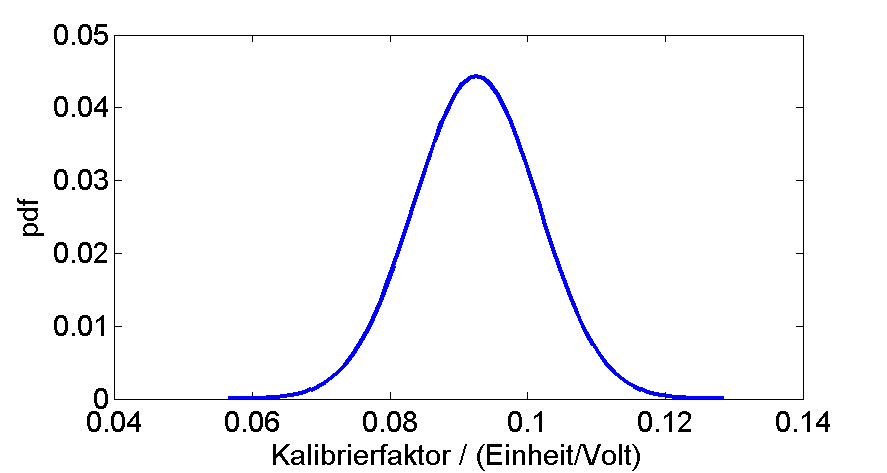
\includegraphics[width=100mm]{Bilder/Kalibrierfaktor.eps}
		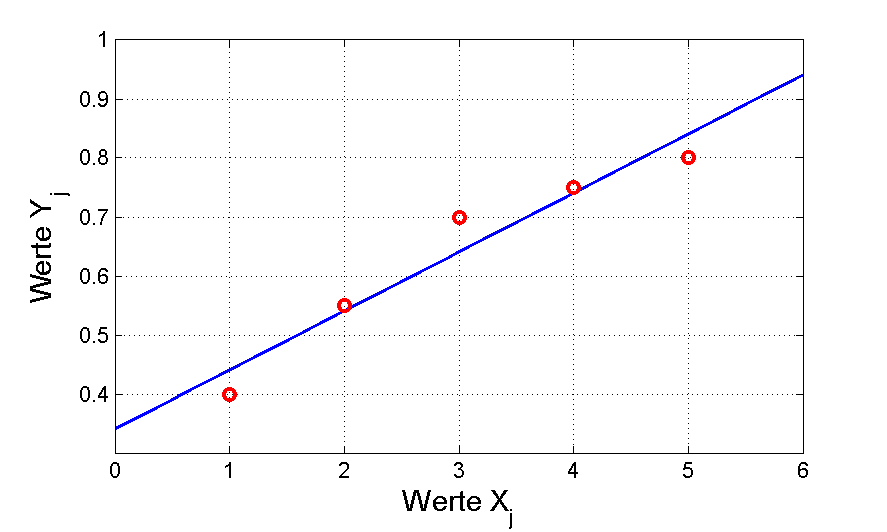
\includegraphics[width=140mm]{02_vorlesung/media/LinRegression.png}
		\caption{Lineare Regression. 
			Als Schätzparameter erhält man $\hat{\boldsymbol\theta} = [ 0.3400 ,0.1000 ]^T$}
		\label{fig:LineareRegression}
	\end{center}
\end{figure}
Die Varianz der Residuen ist wie folgt gegeben:
\begin{equation}
\operatorname{Var}(\epsilon) = \frac{1}{J-M} \cdot \left(\mathbf Y - \mathbf X \hat{\boldsymbol\theta}\right)^T 
\left(\mathbf Y - \mathbf X \hat{\boldsymbol\theta}\right)
\end{equation}
Die Kovarianzen der Schätzerparameter ${\boldsymbol\theta}$ 
sind gegeben durch:
\begin{equation}
\operatorname{Cov}(\boldsymbol\theta) = \left(\mathbf{X}^T \mathbf X \right)^{-1}
\operatorname{Var}(\epsilon)
\end{equation}
Matlab-Code zur Bestimmung des Qualitätsmaßes und der Varianz
\begin{verbatim}
% Qualitätsmaß Q
Q = (Y-X*thetaHat)' * (Y-X*thetaHat)
% Varianz der Residuen
Var_epsilon = 1/df *(Y-X*thetaHat)' * (Y-X*thetaHat)
% Wuzel aus Var_epsilon
RMSE = sqrt(Var_epsilon)
% Kovarianzen
Cov = Var_epsilon * inv(X'*X)
\end{verbatim}
Als Ergebnis für unser Beispiel erhalten wir:\\
Q = 0.0070 \\
Var\_epsilon = 0.0023\\
RMSE = 0.0483 \\
Cov = \\
0.0026   -0.0007 \\
-0.0007    0.0002 \\

\subsection{Fit einer kubischen Funktion (Polynom 3. Ordnung)}
Wir nehmen wieder die gleichen Messwertpaare wie eben. Jedoch fitten wir 
nun eine kubische Funktion durch die Messdaten, d.h. 
\begin{equation}
Y = \hat{\theta_3} X^3 + \hat{\theta_2} X^2 + \hat{\theta_1} X^1 +
\hat{\theta_0} 
\end{equation}
Für die Schätzparameter erhalten wir: 
\[\hat{\boldsymbol\theta} = 
(0.1900, \;\; 0.2286,\;\; -0.0214, \;\; -0.0000) \]
Für das Qualitätsmaß ergibt sich: 
\[\mathrm{Q} = 5.7143e-04 \]
Für die Streuung der Residuen ergibt sich: 
\[\mathrm{Var\_epsilon} = 5.7143e-04 \]
Standardabweichung der Residuen: 
\[
\mathrm{RMSE} = 0.0239 \]
Die Kovarianzamtrix ergibt sich zu: 
\[
\operatorname{Cov} =
\begin{bmatrix}
0.0138  & -0.0176  &  0.0063  & -0.0007 \\
-0.0176 &   0.0236 &  -0.0087 &  0.0009 \\
0.0063  &  -0.0087 &   0.0033 &  -0.0004 \\
-0.0007 &   0.0009 &  -0.0004  &  0.0000
\end{bmatrix}
\]
Der Matlab/Octave-Code lautet: 
\begin{verbatim}
close all; clear all;
% Eingabe der Messwertepaare
input = [...                 
1, 0.4;...                
2, 0.55;...
3, 0.7;...
4, 0.75; ...
5, 0.8];
m = length(input);     % Anzahl der Messpunkte
x_Werte = input(:,1);
X = [ones(m,1), x_Werte, x_Werte.^2,x_Werte.^3];   % Aufstellen der X-Matrix
Y = input(:,2);                % Aufstellen der Y-Matrix
% degree of freedom 
df = 5-4;
% Berechung der Schätzwerte \thetaHat; 
% y-Abschnitt = \thetaHat(1); Steigung = \thetaHat(2)
thetaHat = (X' * X) \ (X' * Y);    
% Anzeige der Schätzwerte
disp(thetaHat);
% Plotten der Fitfunktion
xx = linspace(0,6,100);
yy = thetaHat(1) + thetaHat(2)*xx+ thetaHat(3)*xx.^2+thetaHat(4)*xx.^3;
figure(10)
plot(xx, yy,'linewidth',1.5)
% Plotten der Datenwerte 
hold on
plot(input(:,1), input(:,2), 'or','linewidth',2, 'MarkerSize',6)
hold off
grid on; 
xlabel('Werte X_j','fontsize',14)
ylabel('Werte Y_j','fontsize',14)
set(gcf, 'PaperUnits', 'centimeters');
x_width=15 ;y_width= 9;
set(gcf, 'PaperPosition', [0 0 x_width y_width]);
print '-dpng' kubischerFit.png
% Qualitätsmaß Q
Q = (Y-X*thetaHat)' * (Y-X*thetaHat)
% Varianzen der Residuen
Var_epsilon = 1/df *(Y-X*thetaHat)' * (Y-X*thetaHat)
% Wuzel aus Var_epsilon
RMSE = sqrt(Var_epsilon)
% Kovarianzen
Cov = Var_epsilon * inv(X'*X)
\end{verbatim}
Wir können auch die Curve Fitting Toolbox von Matlab 
verwenden, die uns das gleiche Ergebnis anzeigt:
\begin{figure}[!htp]
	\begin{center}
		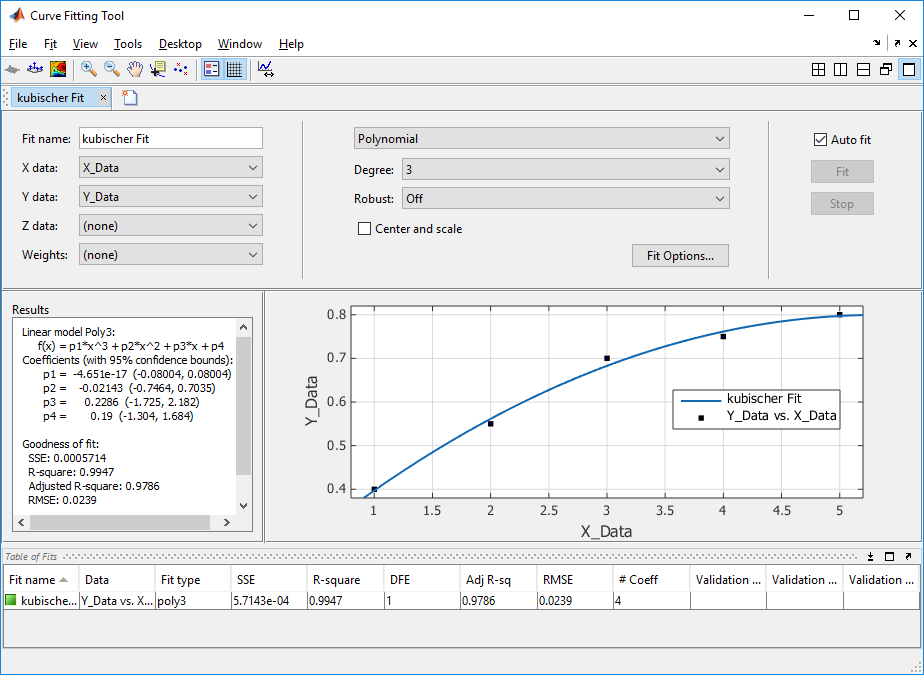
\includegraphics[width=150mm]{02_vorlesung/media/Matlab_CFTool_Kubischer_Fit.png}
		\caption{Kubischer Fit mit der Curve Fitting Toolbox von Matlab. 
			Zum jedem geschätzten Parameter wird der 95\%ige Vertrauensbereich 
			angegeben. Zu sehen sind u.a. das Qualitätsmaß Q (engl. SSE: Sum squared error), das Bestimmtheitsmaß $\rho^2_{XY}$ (engl. R-square), Standardabweichung der Residuen (engl. RMSE: root mean square error) und die Anzahl der Freiheitsgrade (engl. DFE, degree of freedom)}
		\label{fig:CFTool_kubischerFit}
	\end{center}
\end{figure}
\newpage

%Das vollständige Messergebnis für jeden der Regressionparameter ist damit
%\begin{equation}
%\theta_l \; = \;
%\boldsymbol{e}_l^\mathsf{T} \, \left( \mathbf{X}^\mathsf{T}  \, \mathbf{X} \right)^{-1} %\mathbf{X}^\mathsf{T} \, \mathbf{Y}
%\; \pm \; t_{1-\alpha/2, \nu} \, \hat \sigma_l
%\end{equation}
%mit $\nu = J-M$ und die Korrelationskoeffizienten für die Korrelation der %Regressionsparameter
%untereinander sind
%\begin{equation}
%\rho_{l,m} \; = \; \frac{\hat \sigma_{\varepsilon}^2}{\hat \sigma_l \, \hat \sigma_m} \; %\boldsymbol{e}_l^\mathsf{T} \, \left( \mathbf{X}^\mathsf{T}  \, \mathbf{X} \right)^{-1} %\, \boldsymbol{e}_m  .
%\end{equation}

\section{Aufgaben zum Selbststudium}
\subsection{1. Aufgabe zur Linearen Regression}
\label{Vorl2Regressionsaufg1}
Es wurde eine Stufe vermessen, die nominal eine Höhe von $100 \; \mathrm{\mu m}$ haben soll.
Die laterale Achse $x$ wird eingestellt (mit Präzisionstisch positioniert) 
und als Regressor betrachtet, also nicht als Zufallszahl.
Die vertikale Achse $z$ wird gemessen, als Regressand und damit als Zufallszahl
betrachtet.

\begin{center}
	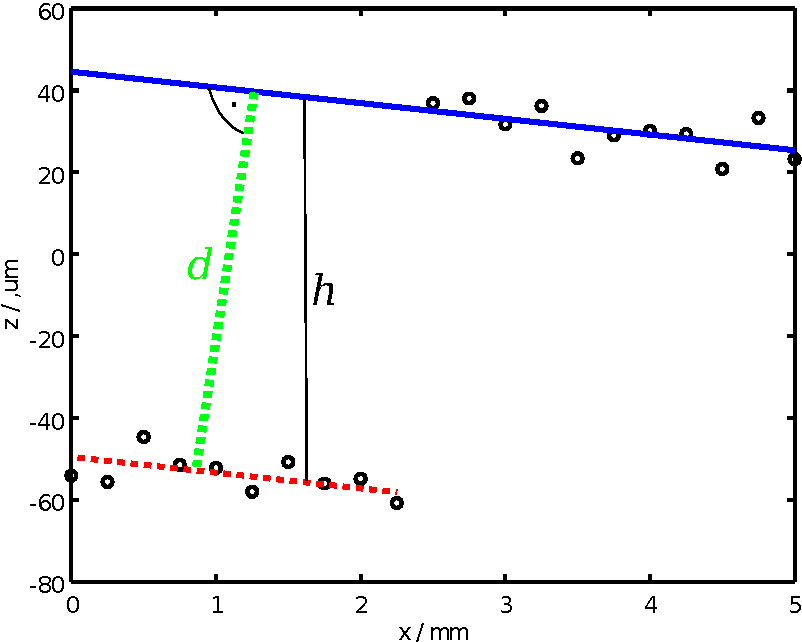
\includegraphics[width=90mm]{02_vorlesung/media/uebungA5_step_plot.pdf}
\end{center}

%\vspace{2mm}

\begin{tabular}{l|c|c|c|c|c|c|c|c|c|c}
	\hline
	$x / \mathrm{mm}$ &
	0.00 & 0.25 & 0.50 & 0.75 & 1.00 & 1.25 & 1.50 & 1.75 & 2.00 & 2.25 \\
	\hline
	$z / \mathrm{\mu m}$ &
	-54.08 &-55.63 &-44.65 &-51.44 &-52.21 &-58.01 &-50.76 &-56.01 &-54.86 &-60.77\\ 
	\hline
\end{tabular}

\vspace{2mm}

\begin{tabular}{l|c|c|c|c|c|c|c|c|c|c|c}
	\hline
	$x / \mathrm{mm}$  & 2.50 &
	2.75 & 3.00 & 3.25 & 3.50 & 3.75 & 4.00 & 4.25 & 4.50 & 4.75 & 5.00 \\
	\hline
	$z / \mathrm{\mu m}$ &36.85 &38.02 &31.71 &36.21 &23.39 &29.01 &30.11 &29.35 &20.81 &33.27 &23.19\\
	\hline
\end{tabular}

\vspace{2mm}

Die Modellgleichung, mit der die Stufe beschrieben wird, ist
$$
z_j \; = \; a \, x_j \, + \, c \, + \, h \, \delta_{j \in C} \; + \; \varepsilon_j
$$
mit $C$ Menge der Indizes von 1 bis $J_C$. Hier sei $J_C = 10$:
$$
C \; = \; \{\, j \, | \, j = 1, 2, \dots, J_C \}
$$
und
$$
\delta_{j \in C} \; = \; \left\{
\begin{array}{ll}
1 & \mathrm{falls} \; \;  j \in C \; \mathrm{~d.h.~} j = 1 \; \mathrm{~oder} \; j = 2
\mathrm{~oder} \; \dots \; j = J_C\\
0 & \mathrm{sonst}
\end{array} \right.
$$
Dabei ist $h$ noch nicht die Stufenhöhe, sondern deren Projektion auf die vertikale Achse.
Die Stufenhöhe $d$ ist der senkrechte Abstand zwischen den beiden parallelen Geraden, die jeweils durch die Punkte auf dem oberen und dem unteren Niveau gehen.

\begin{itemize}
	\item[a)] Stellen Sie das lineare Gleichungssystem auf, das sich durch partielles Ableiten
	für das Optimierungsproblem
	$$
	\min\limits_{a,c,h} \left\{\sum_{j=1}^{J_T} \varepsilon_j^2\right\}
	$$
	ergibt, mit $J_T = 21$.
	\item[b)] Schreiben Sie die Gleichung für die Stufenhöhe $d$ als Funktion von $h$ und $a$ auf.
	\item[c)] Schreiben Sie die Gleichung für die Varianz der Residuen auf.
	\item[d)] Schreiben Sie die Formel für die Kovarianzmatrix der Modellparameter
	$a, c, h$ auf.
	\item[e)] Verwenden Sie eine Programmierumgebung Ihrer Wahl, Matlab, Octave, Python, R, ...
	die Ihnen einen Solver für lineare Gleichungssysteme zur Verfügung stellt, sowie
	eine Routine zur Matrixinversion und berechen Sie die Zahlenwerte für die Modellparameter
	sowie deren Kovarianzmatrix.
\end{itemize}
Anmerkung: Die inverse Matrix brauchen Sie nicht analytisch zu berechnen, sondern
	lediglich $(...)^{-1}$ zu notieren




